%! TEX root = **/010-main.tex
% vim: spell spelllang=en:

\section{Description of pre-processing of data}%
\label{sec:desc-prep}

% Kind of preprocessing done to the original data:  Have you simplified the dataset?
% Removed some examples?
% Feature selection done?
% Did you enrich your dataset with other columns or more information?
% Imputing/removing missing values? 
% Simplification of values? 
% Normalization? 
% Remember that you should describe the all procedures performed on your raw dataset.

\begin{figure}[H]
    \centering
    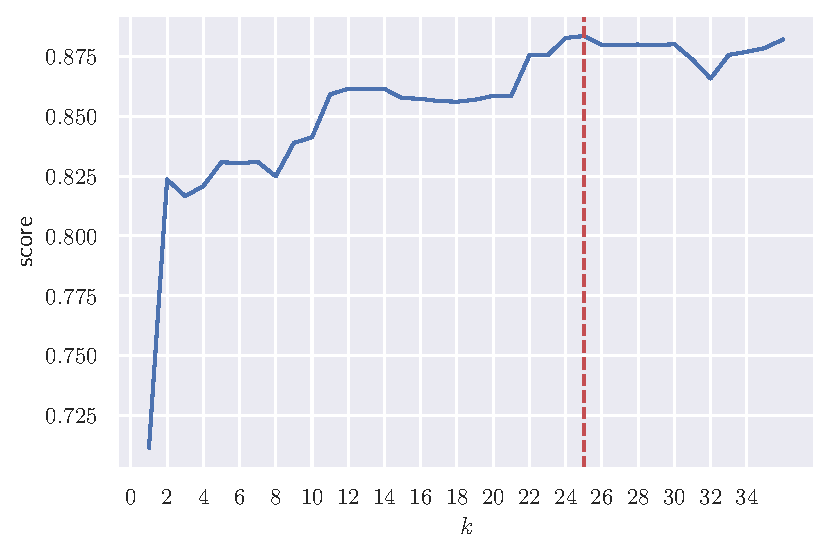
\includegraphics{kbest}
    \caption{Cross validation score for different $k$ values}%
    \label{fig:feature_cross}
\end{figure}

\begin{table}[H]
    \centering
    \caption{Selected features (25)}%
    \label{tab:features}
    \begin{tabular}{lr}
\toprule
                     Variable &     Score \\
\midrule
    \texttt{koi\_steff\_err1} &  0.187327 \\
           \texttt{koi\_prad} &  0.183411 \\
    \texttt{koi\_steff\_err2} &  0.172951 \\
     \texttt{koi\_prad\_err1} &  0.159601 \\
 \texttt{koi\_duration\_err2} &  0.157072 \\
 \texttt{koi\_duration\_err1} &  0.155455 \\
     \texttt{koi\_prad\_err2} &  0.153358 \\
     \texttt{koi\_srad\_err1} &  0.137056 \\
     \texttt{koi\_model\_snr} &  0.135153 \\
         \texttt{koi\_period} &  0.128600 \\
  \texttt{koi\_time0bk\_err1} &  0.125205 \\
  \texttt{koi\_time0bk\_err2} &  0.124540 \\
    \texttt{koi\_slogg\_err2} &  0.123757 \\
    \texttt{koi\_slogg\_err1} &  0.119153 \\
          \texttt{koi\_steff} &  0.115552 \\
   \texttt{koi\_period\_err2} &  0.110208 \\
   \texttt{koi\_period\_err1} &  0.108851 \\
    \texttt{koi\_insol\_err2} &  0.106811 \\
          \texttt{koi\_depth} &  0.106059 \\
    \texttt{koi\_insol\_err1} &  0.105953 \\
            \texttt{koi\_teq} &  0.102837 \\
          \texttt{koi\_insol} &  0.101366 \\
         \texttt{koi\_impact} &  0.100266 \\
           \texttt{koi\_srad} &  0.099673 \\
                 \texttt{dec} &  0.099518 \\
\bottomrule
\end{tabular}

\end{table}